%% 
%% Copyright 2019-2024 Elsevier Ltd
%% 
%% This file is part of the 'CAS Bundle'.
%% --------------------------------------
%% 
%% It may be distributed under the conditions of the LaTeX Project Public
%% License, either version 1.3c of this license or (at your option) any
%% later version.  The latest version of this license is in
%%    http://www.latex-project.org/lppl.txt
%% and version 1.3c or later is part of all distributions of LaTeX
%% version 1999/12/01 or later.
%% 
%% The list of all files belonging to the 'CAS Bundle' is
%% given in the file `manifest.txt'.
%% 
%% Template article for cas-sc documentclass for 
%% double column output.

\documentclass[a4paper,fleqn]{cas-dc}

% If the frontmatter runs over more than one page
% use the longmktitle option.

%\documentclass[a4paper,fleqn,longmktitle]{cas-sc}

%\usepackage[numbers]{natbib}
%\usepackage[authoryear]{natbib}
\usepackage[authoryear]{natbib}
\usepackage{caption}
\usepackage{lineno}

%%%Author macros
\def\tsc#1{\csdef{#1}{\textsc{\lowercase{#1}}\xspace}}
\tsc{WGM}
\tsc{QE}
%%%

% Uncomment and use as if needed
%\newtheorem{theorem}{Theorem}
%\newtheorem{lemma}[theorem]{Lemma}
%\newdefinition{rmk}{Remark}
%\newproof{pf}{Proof}
%\newproof{pot}{Proof of Theorem \ref{thm}}

\begin{document}
\linenumbers
\let\WriteBookmarks\relax
\def\floatpagepagefraction{1}
\def\textpagefraction{.001}

% Short title
\shorttitle{Sample Overlap in Knowledge Distillation}    

% Short author
\shortauthors{Yi Le}  

% Main title of the paper
\title [mode = title]{Exploring the Impact of Sample Overlap on Knowledge Distillation Regularization}  

% Title footnote mark
% eg: \tnotemark[1]


% Title footnote 1.
% eg: \tnotetext[1]{Title footnote text}


% First author
%
% Options: Use if required
% eg: \author[1,3]{Author Name}[type=editor,
%       style=chinese,
%       auid=000,
%       bioid=1,
%       prefix=Sir,
%       orcid=0000-0000-0000-0000,
%       facebook=<facebook id>,
%       twitter=<twitter id>,
%       linkedin=<linkedin id>,
%       gplus=<gplus id>]

\author[1]{Yi Le}%[<options>]

% Corresponding author indication
\cormark[1]



% Email id of the first author
\ead{138032025014@student.fjnu.edu.cn}



% Credit authorship
% eg: \credit{Conceptualization of this study, Methodology, Software}
\credit{Conceptualization, Methodology, Software, Validation, Formal analysis, Investigation, Data curation, Writing -- original draft, Writing -- review and editing, Visualization}

% Address/affiliation
\affiliation[1]{organization={College of Resource Recycling Science and Engineering, Fujian Normal University},
            city={Fuzhou},
            postcode={350117},
            country={China}}



% Corresponding author text
\cortext[1]{Corresponding author}


% For a title note without a number/mark
%\nonumnote{}

% Here goes the abstract

\begin{abstract}
We study how overlap between teacher and student training sets affects knowledge distillation. We introduce an $\alpha$-overlap framework that continuously varies the fraction of shared samples and evaluate its effect on generalization across five tabular benchmarks and two image benchmarks, using 20 seeds, effect sizes, bootstrap confidence intervals, and Holm-corrected significance tests. Complementary partitioning (low $\alpha$) often reduces the student's generalization gap, with the strongest effect on Glass at near-zero overlap ($\alpha{=}0.2$: $\Delta=-0.056$, 95\% CI $[-0.076,-0.033]$, corrected $p=0.028$), whereas the benefit largely vanishes under full overlap ($\alpha=1$). On the held-out test set, the distilled student improves negative log-likelihood on all datasets while preserving calibration, whereas label smoothing severely degrades calibration; complementary distillation dominates label smoothing on these proper predictive metrics on three of the four original tabular datasets, but the advantage is conditional rather than universal. This effect remains robust across teacher--student allocation ratios, label-smoothing strengths, distillation temperatures, and teacher capacities. These results suggest that data complementarity is a useful but dataset-dependent factor in the regularization effect of knowledge distillation.
\end{abstract}

% Use if graphical abstract is present
%\begin{graphicalabstract}
%\includegraphics{}
%\end{graphicalabstract}



% Keywords
% Each keyword is separated by \sep
\begin{keywords}
 \sep Knowledge distillation
  \sep Data partitioning
   \sep Regularization
   \sep Soft labels
\end{keywords}

\maketitle

% Main text
\section{Introduction}\label{}


Knowledge distillation (KD) has found widespread application in machine learning, improving generalization in data-scarce settings~\citep{hinton2015distillingknowledgeneuralnetwork}. Beyond model compression, KD has been shown to benefit same-capacity students through soft-label regularization~\citep{furlanello2018born}, and it has also been explored in federated learning (FL) settings~\citep{FLzhu}.

However, most existing studies assume that the teacher and student are trained on identical data or on samples drawn from the same training distribution. In practice, this assumption is frequently violated. Data may arrive in sequential batches, requiring an early-deployed teacher to be trained on an initial partition while the student learns from a later one. Alternatively, annotation budgets may force a split between labeled samples used to train the teacher and a disjoint set assigned to the student. The effect of teacher--student data partition overlap on distillation generalization has received limited direct study.

This work addresses a practically relevant question: how does the degree of overlap between teacher and student training data affect the generalization performance of the distilled model? We introduce an $\alpha$-overlap framework, which continuously parameterizes the fraction of shared samples between $D_T$ and $D_S$, ranging from fully complementary datasets ($\alpha=0$) to fully shared datasets ($\alpha=1$). We further examine the effect of the data allocation ratio $\beta = |D_T|/|D_{\mathrm{pool}}|$, which captures realistic scenarios in which the teacher and student datasets differ in size.


\paragraph{Contributions.}

First, we introduce the $\alpha$-overlap framework and show that complementary data partitioning ($\alpha \to 0$) can reduce the student's generalization gap, with the clearest effect on Glass at near-zero overlap ($\alpha{=}0.2$: $\Delta=-0.056$, rank-biserial $r=-0.82$, Holm-corrected $p=0.028$, $n=20$ seeds) and a diminishing benefit as overlap increases. Second, we show that the distilled student improves test negative log-likelihood on all datasets while preserving calibration, so the regularization benefit extends beyond the training--validation gap to proper predictive metrics. Third, we show that this effect is robust to the teacher--student allocation ratio $\beta$ (with a minimum teacher pool required on Digits), to the label-smoothing strength, to the distillation temperature and mixing weight at their predictive optimum, and to teacher capacity. Fourth, we compare complementary KD with label smoothing and show that Distill-S dominates generic soft-target smoothing on NLL and calibration on three of the four original tabular datasets, while label smoothing is stronger on Digits---a conditional, dataset-dependent benefit that tracks how much the teacher disagrees with the student on the student's own data. Finally, we provide an exploratory separability and agreement analysis, which suggests that poor class separability and low teacher--student agreement may favor complementary KD but do not fully explain all outcomes.


\section{Related Work}


\citet{hinton2015distillingknowledgeneuralnetwork}
introduced KD as a training procedure in which a student minimizes
the KL divergence from teacher soft labels alongside a hard-label
cross-entropy term.

\citet{stanton2021does}
subsequently questioned whether KD reliably transfers teacher
knowledge, finding that student fidelity to the teacher does not
always improve generalization. Our work provides a complementary
perspective: we show that the \emph{informational overlap} between
teacher and student training sets is a key factor mediating
distillation benefit, offering a possible perspective on why
self-distillation on identical data may fail to improve generalization.


In federated learning, raw data cannot be shared across clients;
\citet{FLzhu} proposed data-free KD as a
communication-efficient alternative, where soft labels are exchanged
instead of gradients. While our training procedure follows the same distillation principle, our focus differs: rather than treating data heterogeneity as an obstacle to overcome, we treat it as a controlled variable and characterize its effect on generalization.

Closer to our setting, Hierarchical Self-supervised Augmented KD
\citep{yang2021hierarchical} augments the teacher's supervision with
hierarchical self-supervised signals, and MixSKD \citep{yang2022mixskd}
distills self-knowledge from mixup-augmented views; both enrich the
\emph{information content} of the transferred targets, whereas we hold the
transfer mechanism fixed and vary only the overlap between teacher and
student training sets.

We emphasize the scope of the contribution: the $\alpha$-overlap framework
is a controlled data-partitioning \emph{protocol} for isolating the effect
of teacher--student data complementarity, not a new distillation method.
Its value is diagnostic---quantifying when soft labels carry information
beyond the student's own training data---and the resulting observations
complement existing work on self-distillation \citep{furlanello2018born},
data-free federated distillation \citep{FLzhu}, and soft-target
regularization \citep{szegedy2016rethinking}.

\section{Method}

\subsection{Notation}

Let $P$ denote the full dataset, which is first split into a training set $D$ and a test set at an 8:2 ratio. We further reserve 20\% of the training samples as the validation set $D_{val}$; the remaining samples form $D_{pool}$, with size $N = |D_{pool}|$. The core notation is as follows:

\begin{itemize}
  \item $D_S$: Training set for student, size $|D_S| = (1-\beta) * N$

  \item $D_T$: Training set for teacher, size $|D_T| = \beta * N$

  \item $\alpha \in [0,1]$ The overlapping ratio of $D_S$ and $D_T$, $\alpha = \frac{|D_S \cap D_T|}{|D_S|}$

  \item $\beta \in [0,1] $ = $|D_T| / |D_{pool}|$

  \item $\lambda$: The mixing weight of soft labels and hard labels in the distillation loss is fixed at $\lambda = 0.5$ in this experiment.


\end{itemize}


\subsection{Experimental Design}

\textbf{Experiment 1 ($\alpha$-sweep).}
We fix $\beta = 0.5$ (i.e., $|D_T|=|D_S|=N/2$) and sweep
$\alpha \in \{0.0, 0.2, 0.4, 0.6, 0.8, 1.0\}$.
For each $\alpha$, $D_T$ is constructed by taking
$\lfloor \alpha \cdot N/2 \rfloor$ samples from $D_S$
(the overlapping portion) and sampling the remaining
$N/2 - \lfloor \alpha \cdot N/2 \rfloor$ samples from the
complementary pool half (the non-overlapping portion),
using a seed determined jointly by the random seed and $\alpha$
to prevent nested-subset bias across conditions.
Three groups are compared at each $\alpha$:
\textbf{Baseline-Full} trains on the entire pool with hard labels
(upper bound);
\textbf{Baseline-Half} trains on $D_S$ with hard labels only
(fair control);
\textbf{Distill-S} trains on $D_S$ with the mixed loss defined below.

\textbf{Construction constraints and class composition.}
Since $\alpha$ is defined relative to $|D_S|$, the design requires
$|D_T| \ge \alpha |D_S|$, i.e.\ $\beta \ge \alpha(1-\beta)$; asymmetric
regimes ($\beta \neq 0.5$ with $\alpha > 0$) are therefore excluded from
the present study---the $\alpha$-sweep fixes $\beta=0.5$ and the
$\beta$-sweep fixes $\alpha=0$, so each sweep varies one factor in a
symmetric regime. $D_S$ is the tail of a seeded random permutation of the
pool, and the non-overlapping part of $D_T$ is drawn from the complementary
pool half with an independent, seed-and-$\alpha$-dependent permutation, so
class composition is balanced only in expectation rather than by exact
stratification; no class is excluded from either partition. Teacher
probabilities are mapped onto the global class index set of the dataset
(via the teacher's fitted \texttt{classes\_} attribute) so that soft-label
columns remain aligned with the student's output dimension even when a
rare class is absent from $D_S$ or $D_T$.

\textbf{Experiment 2 ($\beta$-sweep).}
We fix $\alpha = 0$ (fully disjoint partitions) and sweep
$\beta \in \{0.2, 0.3, \ldots, 0.8\}$ on Breast Cancer and Glass.
The pool is split sequentially: the first $\lfloor\beta N\rfloor$
samples form $D_T$ and the rest form $D_S$.
The per-$\beta$ control is \textbf{Baseline-Student}, which trains
on the same $D_S$ as Distill-S but with hard labels only,
isolating the effect of distillation from varying student set size.

\textbf{Label smoothing baseline.}
To separate the effect of generic soft-target regularization from
teacher-provided complementary information, we additionally train
\textbf{Baseline-LS} on the same $D_S$ as Baseline-Half using label
smoothing~\citep{szegedy2016rethinking} with $\varepsilon=0.1$.
Unlike Distill-S, this baseline receives no instance-specific soft labels
from a teacher trained on complementary data. Therefore, comparing
Distill-S with Baseline-LS at $\alpha=0$ tests whether complementary KD
provides benefits beyond ordinary label-smoothing regularization.

\subsection{Model and Loss}

Both teacher and student share the same MLP topology
(input $\to$ 64 $\xrightarrow{\mathrm{ReLU}}$ 32
$\xrightarrow{\mathrm{ReLU}}$ output), following the
same-architecture distillation paradigm of
Born-Again Networks~\citep{furlanello2018born}.
The teacher is trained with scikit-learn's \texttt{MLPClassifier}
for a fixed 300 iterations without early stopping, producing
calibrated \texttt{predict\_proba} outputs as soft labels ($T=1$).
The student is trained with Adam ($\mathrm{lr}=10^{-3}$,
batch size 32) for up to 300 epochs with early stopping
(patience = 20, monitored on $\mathcal{L}_{\mathrm{val}}$).

The student's training loss is:
\begin{equation}
  \mathcal{L} = \lambda\,D_{\mathrm{KL}}\!\left(
    \mathbf{q}^T \,\|\, \hat{\mathbf{p}}
  \right)
  + (1-\lambda)\,\mathcal{L}_{\mathrm{CE}}(\mathbf{y},\hat{\mathbf{p}})
\end{equation}
where $\mathbf{q}^T$ is the teacher's softmax probability vector,
$\hat{\mathbf{p}}$ is the student's log-softmax output,
and $\lambda = 0.5$. Baseline models use $\mathcal{L}_{\mathrm{CE}}$
only.

\subsection{Evaluation Metrics}

Metrics are recorded per run on three disjoint sample sets:

\begin{itemize}
  \item \textbf{best\_val\_acc}: validation accuracy at the epoch
        of minimum $\mathcal{L}_{\mathrm{val}}$, measuring peak
        generalization performance.
  \item \textbf{final\_gen\_gap}:
        $\mathrm{acc}_{\mathrm{train}} - \mathrm{acc}_{\mathrm{val}}$
        at the final training epoch, measuring the degree of
        overfitting.
  \item $e^*$: the epoch index at which $\mathcal{L}_{\mathrm{val}}$
        reaches its global minimum, serving as a proxy for the
        onset of overfitting; a larger $e^*$ indicates delayed
        overfitting.
  \item \textbf{Test metrics}: accuracy and negative log-likelihood
        (NLL) on the held-out test set, evaluated at the best-validation
        checkpoint. Because the validation set drives early stopping,
        test metrics are the primary evidence for predictive
        generalization; the generalization gap is reported as a
        complementary \emph{mechanistic} indicator of regularization.
  \item \textbf{Calibration}: expected calibration error (ECE) with 15
        equal-width confidence bins at the same checkpoint.
\end{itemize}

Statistical analysis follows a paired-by-seed design over $n=20$ random
seeds. For each contrast we report the Wilcoxon signed-rank two-sided
$p$-value, a bootstrap 95\% confidence interval for the paired mean
difference (10{,}000 resamples), and the rank-biserial effect size $r$.
Because each contrast family spans multiple datasets and sweep values,
within-family $p$-values are corrected with Holm's step-down procedure;
we mark significance at Holm-adjusted $p<0.05$.

\section{Experiment}

\subsection{Dataset}

Experiments are conducted on four UCI benchmark classification tabular
datasets: Wine (178 samples, 13 features, 3 classes)~\citep{wine},
Breast Cancer Wisconsin (569 samples, 30 features, 2
classes)~\citep{breastcancer}, Digits (1797 samples, 64 features,
10 classes)~\citep{sklearn}, and Glass Identification (214 samples, 9 features,
6 classes)~\citep{glass}. Wine, Breast Cancer, and Digits are loaded via scikit-learn~\citep{sklearn};
Glass is retrieved from the UCI Machine Learning
Repository~\citep{uci} via \texttt{fetch\_openml}.
Table~\ref{tab:datasets} summarizes the four datasets. As an additional
difficulty probe (Section~\ref{sec:sep}) we also use Yeast (1{,}484
samples, 8 features, 10 classes)~\citep{yeast}, which is markedly harder
for the same MLP protocol.

\begin{table}[h]
  \centering
  \small
  \caption{Summary of the benchmark datasets used in the experiments.}
  \label{tab:datasets}
  \begin{tabular}{lccc}
    \toprule
    Dataset & Samples & Features & Classes \\
    \midrule
    Wine & 178 & 13 & 3 \\
    BreastCancer & 569 & 30 & 2 \\
    Digits & 1797 & 64 & 10 \\
    Glass & 214 & 9 & 6 \\
    \bottomrule
  \end{tabular}
\end{table}

\subsection{Effect of Data Overlap}
\label{Effect}



Figure~\ref{fig:alpha_vs_gengap} reports mean final generalization gap
of Distill-S and Baseline-Half across $\alpha \in
\{0.0,0.2,0.4,0.6,0.8,1.0\}$ on four datasets ($n=20$ seeds,
error bars = $\pm$1 std).

\begin{figure*}[t]
  \centering
  \includegraphics[width=0.98\textwidth]{figure_1.png}
  \caption{Final generalization gap versus overlap ratio $\alpha$. Lower values indicate less overfitting; significance markers denote Wilcoxon signed-rank tests against Baseline-Half. Red annotations show the difference from Baseline-Half.}
  \label{fig:alpha_vs_gengap}
\end{figure*}

Overall, smaller overlap generally leads to a smaller generalization gap for Distill-S, with Wine as the main exception. On Breast Cancer, Distill-S stays below the Baseline-Half gap across all $\alpha$ values, ranging from $0.0214$ at $\alpha{=}0.0$ to $0.0283$ at $\alpha{=}1.0$, compared with $0.0288$ for Baseline-Half. The effect is therefore consistent but small. On Digits, the gain is concentrated at full complementarity: the gap drops from $0.0418$ to $0.0321$ at $\alpha{=}0.0$ ($\Delta=-0.0097$), then gradually approaches the baseline as $\alpha$ increases. Glass shows the strongest dependence on overlap. At $\alpha{=}0.2$, Distill-S reduces the gap from $0.2012$ to $0.1454$ ($\Delta=-0.0558$, bootstrap 95\% CI $[-0.076,-0.033]$, rank-biserial $r=-0.82$, Holm-adjusted $p=0.028$), but this advantage quickly disappears as overlap grows; at $\alpha{=}1.0$, Distill-S slightly exceeds Baseline-Half. This pattern suggests that soft labels are most useful when the teacher contributes information from samples not already seen by the student. On Wine, the changes are negligible ($\Delta \in [-0.007, 0.000]$, all Holm-adjusted $p>0.05$), likely because the dataset is nearly linearly separable and can already be learned well from a random half-split.


Figure~\ref{fig:curves} shows the generalization gap as a function of training epoch.

\begin{figure*}[t]
  \centering
  \includegraphics[width=0.86\textwidth]{figure_2.png}
  \caption{Mean generalization gap over training epochs. Shaded bands denote $\pm$1 std over 20 seeds. Red and orange show Distill-S with $\alpha{=}0.0$ and $\alpha{=}1.0$, respectively; green dashed shows Baseline-Half.}
  \label{fig:curves}
\end{figure*}

These curves suggest that teacher soft labels slow convergence relative to hard-label training. Across the four datasets, Distill-S with either $\alpha=0.0$ or $\alpha=1.0$ generally requires at least as many epochs as the hard-label baseline. More importantly, the $\alpha=0.0$ curve stays below Baseline-Half from approximately epoch 20 onward, indicating that its lower generalization gap is not caused by a late-stage improvement but by a consistently more regularized training trajectory.

\subsection{Test-Set Performance and Calibration}
\label{sec:test}

Because the generalization gap can shrink either because validation
performance improves or because training accuracy is suppressed, we
evaluate the best-validation checkpoint on the held-out test set
(Table~\ref{tab:test_metrics}).

\begin{table*}[t]
\centering
\caption{Test-set performance at $\alpha{=}0$ (fully complementary
         partition), averaged over 20 seeds at the best-validation
         checkpoint. Baseline-Full uses the entire pool and is an upper
         bound rather than an equal-data control. Bold marks the best
         value among the equal-data groups (Baseline-Half, Baseline-LS,
         Distill-S). Distill-S vs.\ Baseline-LS: NLL and ECE differences
         on Wine, Breast Cancer, and Digits are significant at
         Holm-adjusted $p<0.001$ ($r \ge 0.91$); on Glass neither metric
         separates the two. Distill-S vs.\ Baseline-Half: NLL differences
         are negative on all four datasets but not significant after
         Holm correction.}
\label{tab:test_metrics}
\setlength{\tabcolsep}{4.5pt}
\begin{tabular}{l cccc cccc cccc}
\toprule
 & \multicolumn{4}{c}{Test accuracy $\uparrow$}
 & \multicolumn{4}{c}{NLL $\downarrow$}
 & \multicolumn{4}{c}{ECE $\downarrow$} \\
Group & Wine & BC & Dig. & Glass
      & Wine & BC & Dig. & Glass
      & Wine & BC & Dig. & Glass \\
\midrule
Baseline-Half & 0.964 & 0.967 & 0.953 & 0.617
              & 0.106 & 0.106 & 0.166 & 1.068
              & \textbf{0.048} & \textbf{0.030} & 0.025 & 0.185 \\
Baseline-Full & \textbf{0.978} & \textbf{0.972} & \textbf{0.971} & \textbf{0.687}
              & \textbf{0.064} & \textbf{0.105} & \textbf{0.122} & \textbf{0.942}
              & \textbf{0.031} & \textbf{0.028} & \textbf{0.019} & \textbf{0.163} \\
Baseline-LS   & 0.961 & 0.965 & \textbf{0.967} & 0.626
              & 0.169 & 0.133 & 0.250 & \textbf{0.990}
              & 0.116 & 0.070 & 0.134 & \textbf{0.165} \\
Distill-S     & 0.971 & 0.970 & 0.958 & 0.645
              & 0.088 & 0.090 & 0.148 & 1.006
              & 0.050 & 0.032 & \textbf{0.022} & 0.168 \\
\bottomrule
\end{tabular}
\end{table*}

Three observations follow. First, test accuracy: Distill-S slightly exceeds
Baseline-Half on all four datasets (e.g.\ Glass $0.645$ vs.\ $0.617$; Digits
$0.958$ vs.\ $0.953$), though none of these accuracy differences against
Baseline-Half is significant after Holm correction; on Digits it is label
smoothing that leads ($0.967$). Distillation therefore does not buy
accuracy in this equal-data regime---consistent with the regularizer
interpretation---but it also does not trade accuracy away, with LS on Digits
the one group that stays ahead of Distill-S. Second, NLL: Distill-S improves the proper
scoring rule over Baseline-Half on \emph{all four} datasets (e.g.\
Wine $0.088$ vs.\ $0.106$; Digits $0.148$ vs.\ $0.166$), indicating
better-calibrated probabilistic predictions rather than mere
underfitting. Third, calibration: Distill-S preserves the ECE of the
hard-label baselines (e.g.\ Digits $0.022$ vs.\ $0.025$), whereas
Baseline-LS degrades it severely (Digits $0.134$, Wine $0.116$;
Holm-adjusted $p<0.001$, $r=-1.0$ in favor of Distill-S on Wine,
Breast Cancer, and Digits). The comparison with label smoothing is thus
decisive on proper predictive metrics: on three of four datasets,
complementary KD dominates LS well beyond the training--validation gap,
even where accuracy differences are small. On Glass, LS achieves a
slightly better NLL while Distill-S retains the advantage in the
generalization gap, marking Glass as the regime where the two
regularizers are closest.

\subsection{Teacher Quality and Teacher--Student Agreement}
\label{sec:teacher}

At $\alpha{=}0$ the teacher is trained on data fully disjoint from the
student. Mean teacher test accuracy is high on the separable datasets
(Wine $0.965$, Breast Cancer $0.970$, Digits $0.957$) and moderate on
Glass ($0.662$). Teacher calibration and soft-label entropy track the
same difficulty gradient: teacher ECE is $0.021$--$0.047$ on the
separable tabular datasets but rises to $0.227$ on Glass, $0.167$ on
CIFAR-10 and $0.133$ on Yeast, and mean soft-label entropy behaves
analogously ($0.05$--$0.12$ vs.\ $0.46$ on Glass and $0.77$ on Yeast).
Teachers on harder tasks are thus less certain, and their soft labels
carry more distributional information. Two mechanism-level observations
support the
complementarity interpretation. First, the teacher--student agreement
rate on the student's own training samples differs sharply across
datasets: on the separable datasets the student reproduces the teacher's
label on $\ge 96\%$ of $D_S$, so the soft labels act mostly as
confidence smoothing; on Glass agreement is only $77\%$, i.e.\ roughly a
quarter of the teacher's soft labels encode inter-class structure the
student has not recovered from its own data. This gradient tracks the
benefit pattern: complementary KD helps most exactly where the teacher
disagrees most; a quantitative cross-dataset version of this relation
is reported in Section~\ref{sec:sep}. Second, across
all $\alpha$ conditions the distillation
benefit in the generalization gap correlates with teacher quality
(Fig.~\ref{fig:teacher_quality}): pools that induce a stronger teacher
also induce a larger gap reduction, indicating that the effect is not an
artifact of systematically weak teachers.

\begin{figure*}[t]
  \centering
  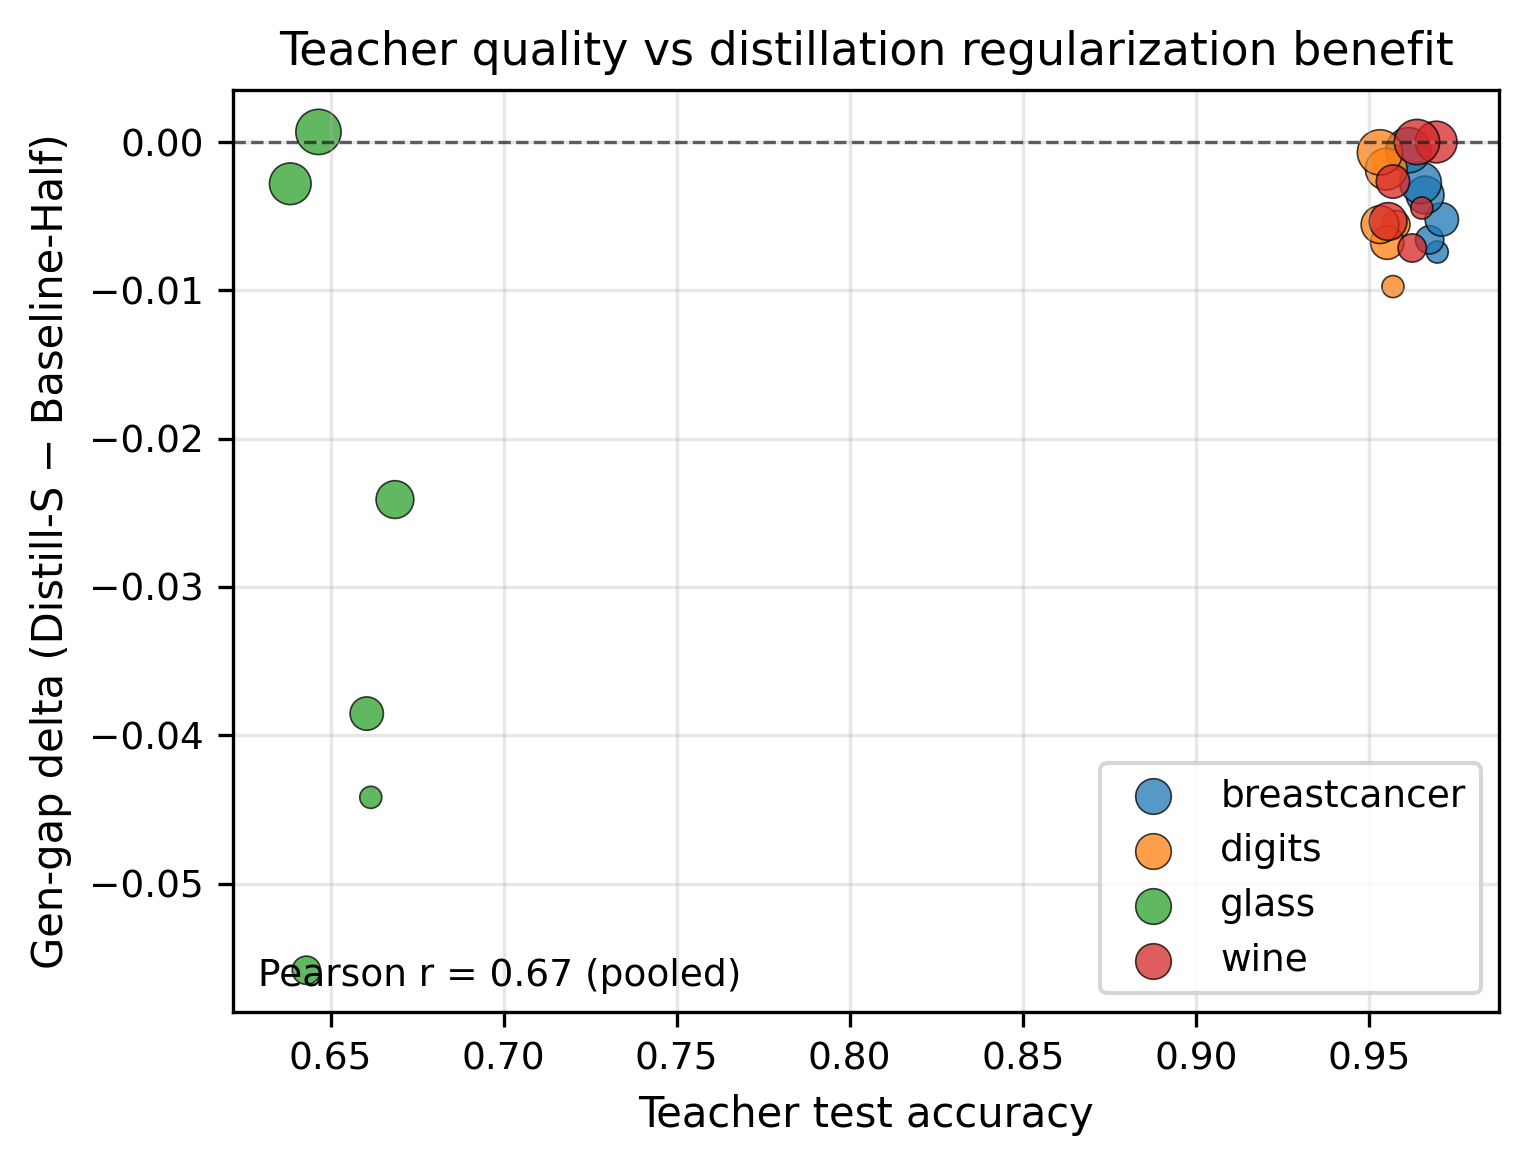
\includegraphics[width=0.62\textwidth]{results_ext/figs/fig_teacher_quality.png}
  \caption{Teacher test accuracy (marker size $\propto \alpha$) versus the
           generalization-gap difference between Distill-S and
           Baseline-Half, pooled over datasets and $\alpha$ values
           ($n=20$ seeds per point). Negative values indicate a smaller
           gap for the distilled student.}
  \label{fig:teacher_quality}
\end{figure*}

\subsection{Hyperparameter Sensitivity and Teacher Capacity}
\label{sec:sensitivity}

To ensure that neither baseline nor treatment benefits from a favorable
hyperparameter choice, we sweep the label-smoothing strength
$\varepsilon \in \{0.05, 0.1, 0.2, 0.3\}$ and the distillation
temperature and mixing weight, $T \in \{1, 2, 4\} \times \lambda \in
\{0.3, 0.5, 0.7\}$, at $\alpha{=}0$ on all four datasets
(Fig.~\ref{fig:sensitivity}). LS behavior is stable across
$\varepsilon$: on Digits, LS remains the stronger regularizer at every
$\varepsilon$ (gap $0.026$--$0.029$), so the Digits result is not an
artifact of $\varepsilon=0.1$. For KD, the gap decreases monotonically
as $\lambda$ or $T$ grows, but test accuracy and NLL degrade sharply on
Glass at the same settings (e.g.\ $T{=}2, \lambda{=}0.5$: gap $0.108$
but test accuracy $0.564$ vs.\ $0.645$ at $T{=}1$). Large-temperature,
soft-label-dominated configurations therefore \emph{buy} a smaller gap
by underfitting---precisely the confound raised about gap-based
evidence, and the reason our conclusions are anchored on test metrics.
The default configuration ($T{=}1$, $\lambda{=}0.5$) used throughout the
study is at the predictive-performance optimum of the swept grid.
Teacher-capacity variants (hidden sizes $(32,16)$, $(64,32)$,
$(128,64)$; student fixed) leave teacher accuracy nearly unchanged on
both capacity-relevant datasets (Glass $0.654$--$0.662$; Breast Cancer
$\approx 0.970$) and do not qualitatively alter the student outcome,
indicating that the reported effects are robust to the tested capacity
range.

\begin{figure*}[t]
  \centering
  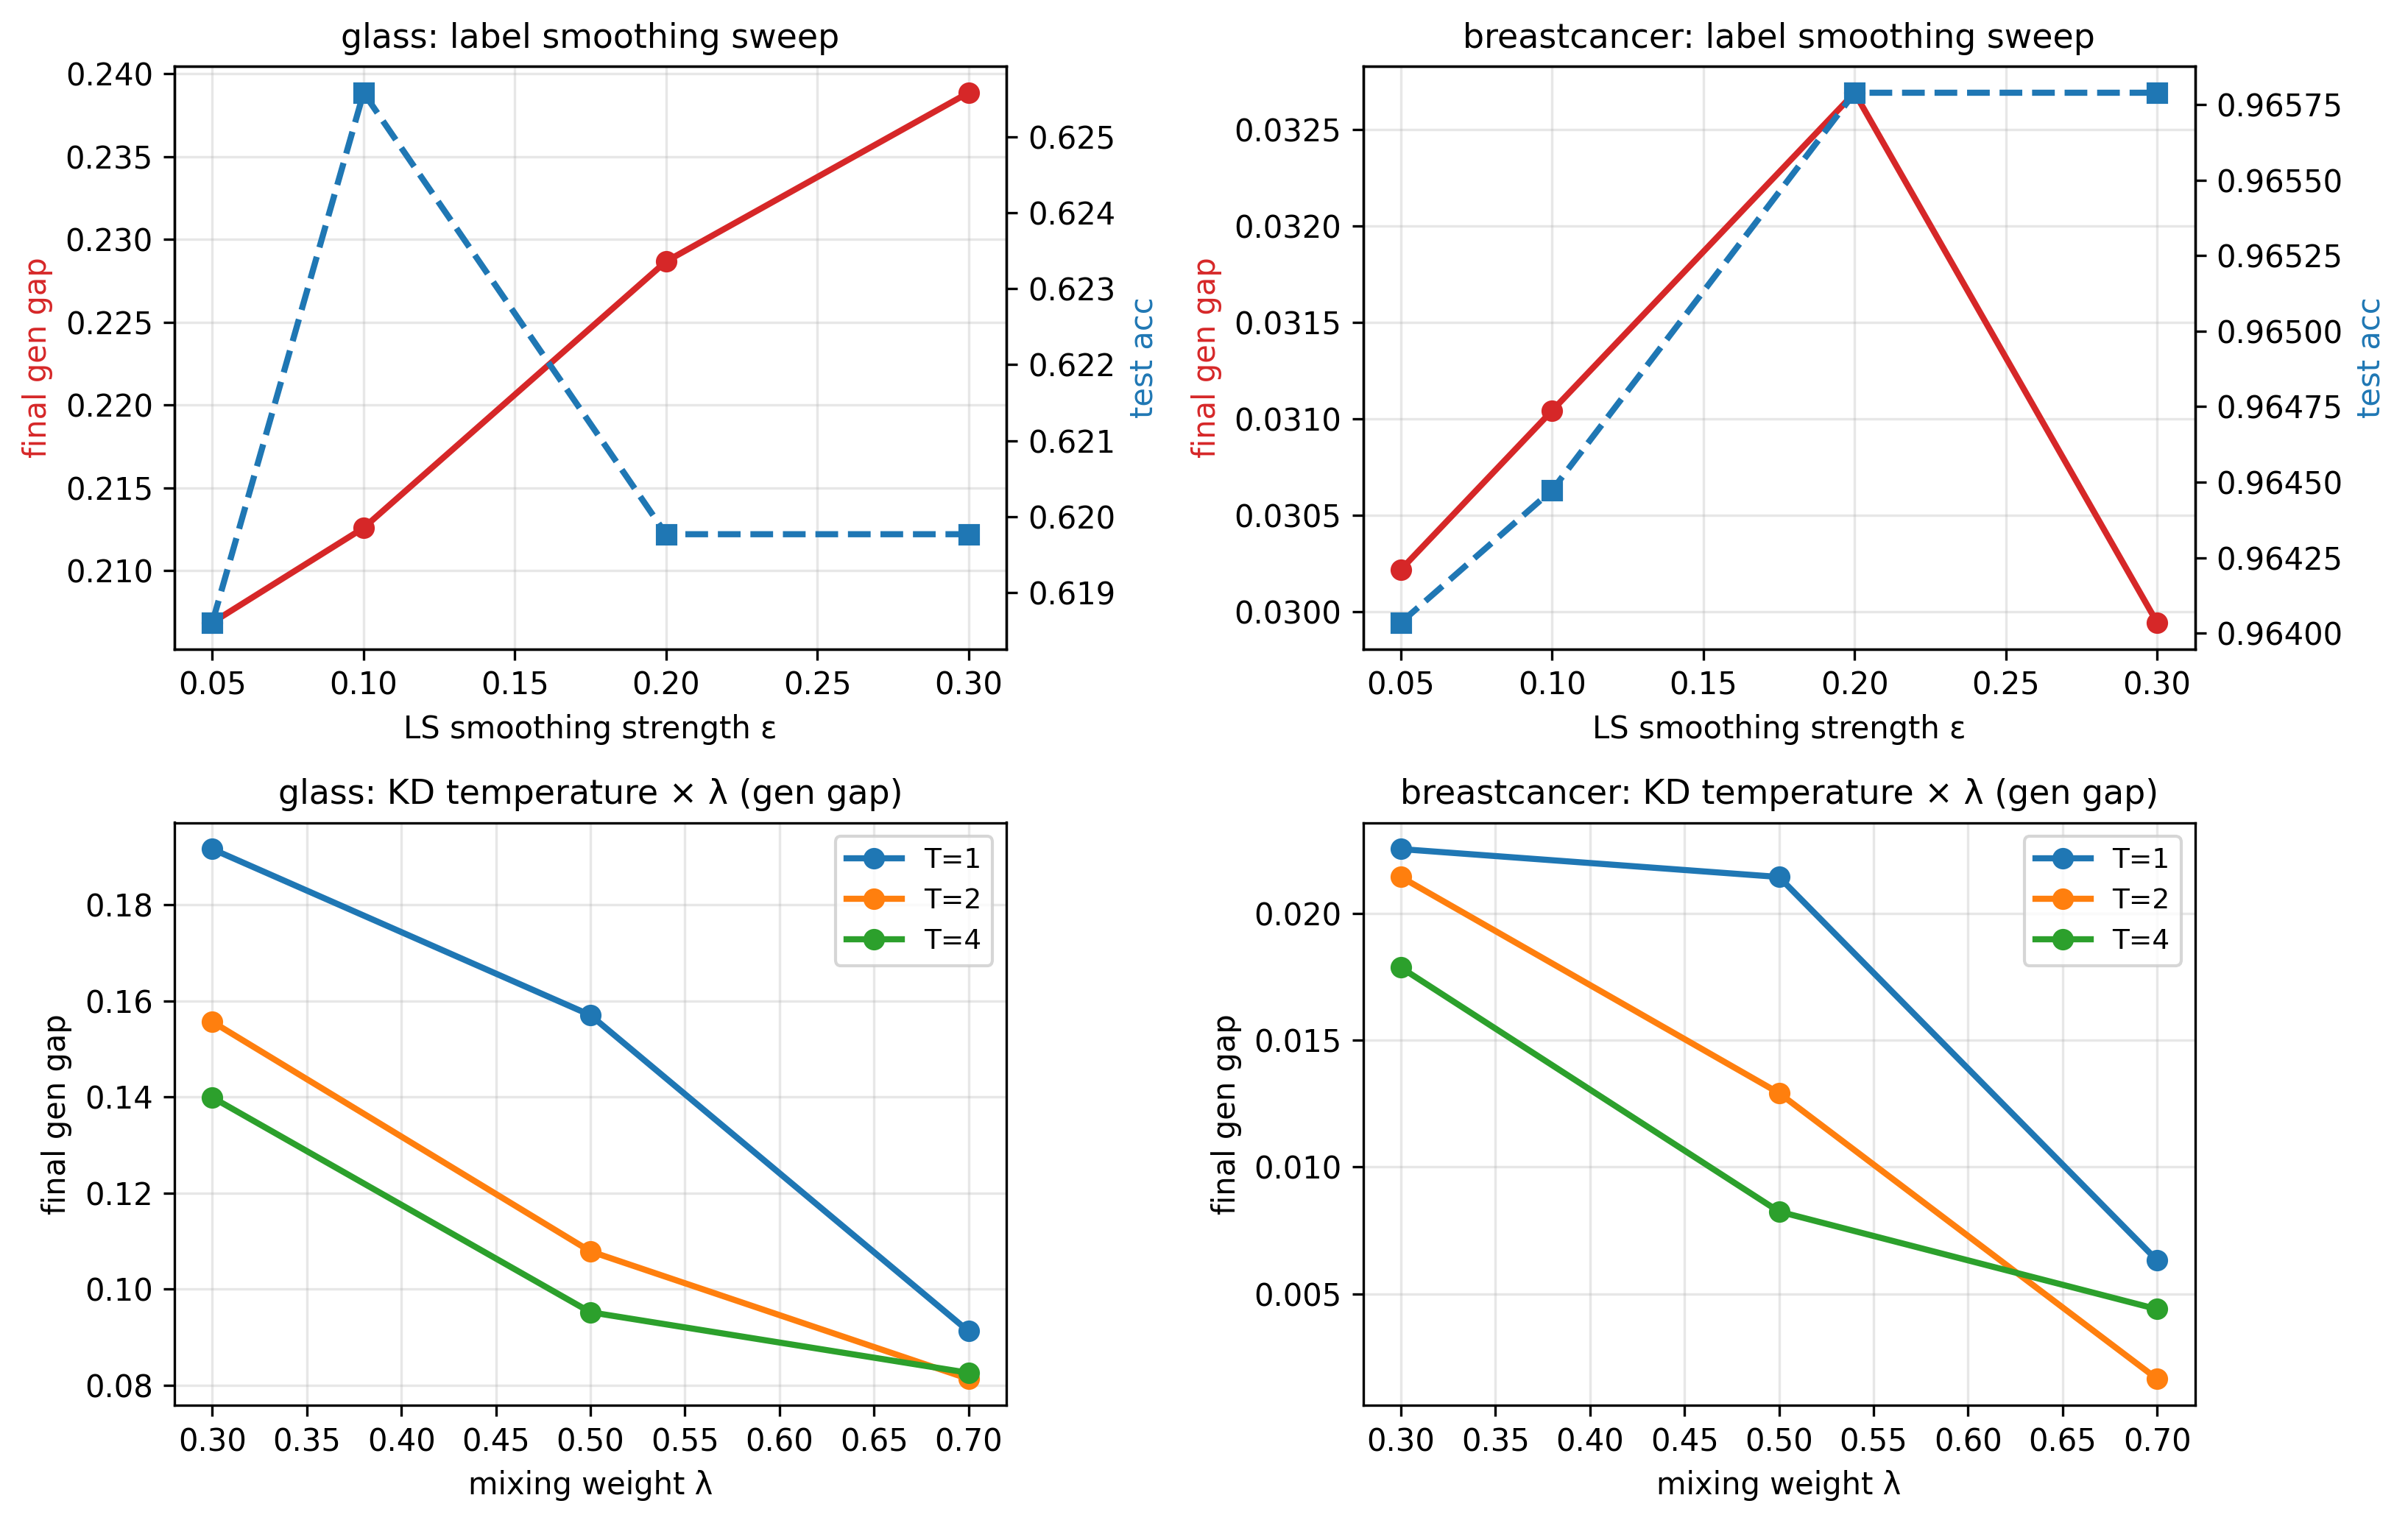
\includegraphics[width=0.95\textwidth]{results_ext/figs/fig_sensitivity.png}
  \caption{Sensitivity of the label-smoothing baseline ($\varepsilon$,
           top) and of distillation ($T \times \lambda$, bottom) at
           $\alpha{=}0$. Left: Glass; right: Breast Cancer.}
  \label{fig:sensitivity}
\end{figure*}

\subsection{Image Benchmarks}
\label{sec:images}

To test whether the observations extend beyond small tabular data, we
repeat the $\alpha$-sweep on Fashion-MNIST and CIFAR-10 using a
three-block VGG-style CNN (channels 32--64--128, batch normalization)
for both teacher and student, 60 fixed teacher epochs, and the official
test splits; all other protocol settings (20 seeds, $\beta=0.5$,
$\lambda=0.5$, $T=1$, $\varepsilon=0.1$, patience 20) are identical to
the tabular study. Figure~\ref{fig:images} reports the final
generalization gap and test accuracy as functions of $\alpha$.

On Fashion-MNIST the tabular findings reappear with a larger effect
size, and---for the first time---with a clear test-accuracy gain. At
$\alpha{=}0$, Distill-S reduces the final generalization gap from
$0.077$ to $0.040$ ($\Delta=-0.038$, 95\% CI $[-0.040,-0.037]$,
Holm-adjusted $p<10^{-4}$, $r=-1.0$), \emph{increases} test accuracy by
$1.1$ points ($0.923$ vs.\ $0.912$; $p<10^{-4}$, $r=1.0$)---matching
the accuracy of Baseline-Full with half of its training data---and
improves test NLL ($0.230$ vs.\ $0.257$, $p<10^{-4}$). All three
advantages decay monotonically with $\alpha$ and are statistically
indistinguishable from Baseline-Half at $\alpha{=}1.0$, while
calibration is preserved throughout ($\mathrm{ECE}\approx 0.02$--$0.03$).
Label smoothing shows the same pathology as on tabular data: it
trades a moderate gap reduction for severely degraded calibration
($\mathrm{ECE}=0.069$) and NLL ($0.306$). On CIFAR-10 the pattern is
amplified further. At $\alpha{=}0$ the final generalization gap drops
from $0.222$ to $0.121$ ($\Delta=-0.101$, 95\% CI $[-0.106,-0.097]$,
Holm-adjusted $p<10^{-4}$, $r=-1.0$)---lower even than that of
Baseline-Full ($0.178$)---and test accuracy rises by $4.4$ points
($0.788$ vs.\ $0.744$; $p<10^{-4}$, $r=1.0$), matching Baseline-Full
($0.794$) with half of its training data; test NLL improves from $0.772$
to $0.665$ ($p<10^{-4}$). Relative to label smoothing, Distill-S is
better on the gap, accuracy, and NLL (all Holm-adjusted $p<10^{-4}$),
although LS yields slightly better calibration on this dataset
($\mathrm{ECE}=0.049$ vs.\ $0.068$). At $\alpha{=}1.0$ none of the
advantages survives, and distilled students fall slightly
\emph{below} Baseline-Half in accuracy, indicating that distilling
from a teacher trained on identical data adds estimation noise rather
than information.

\begin{figure*}[t]
  \centering
  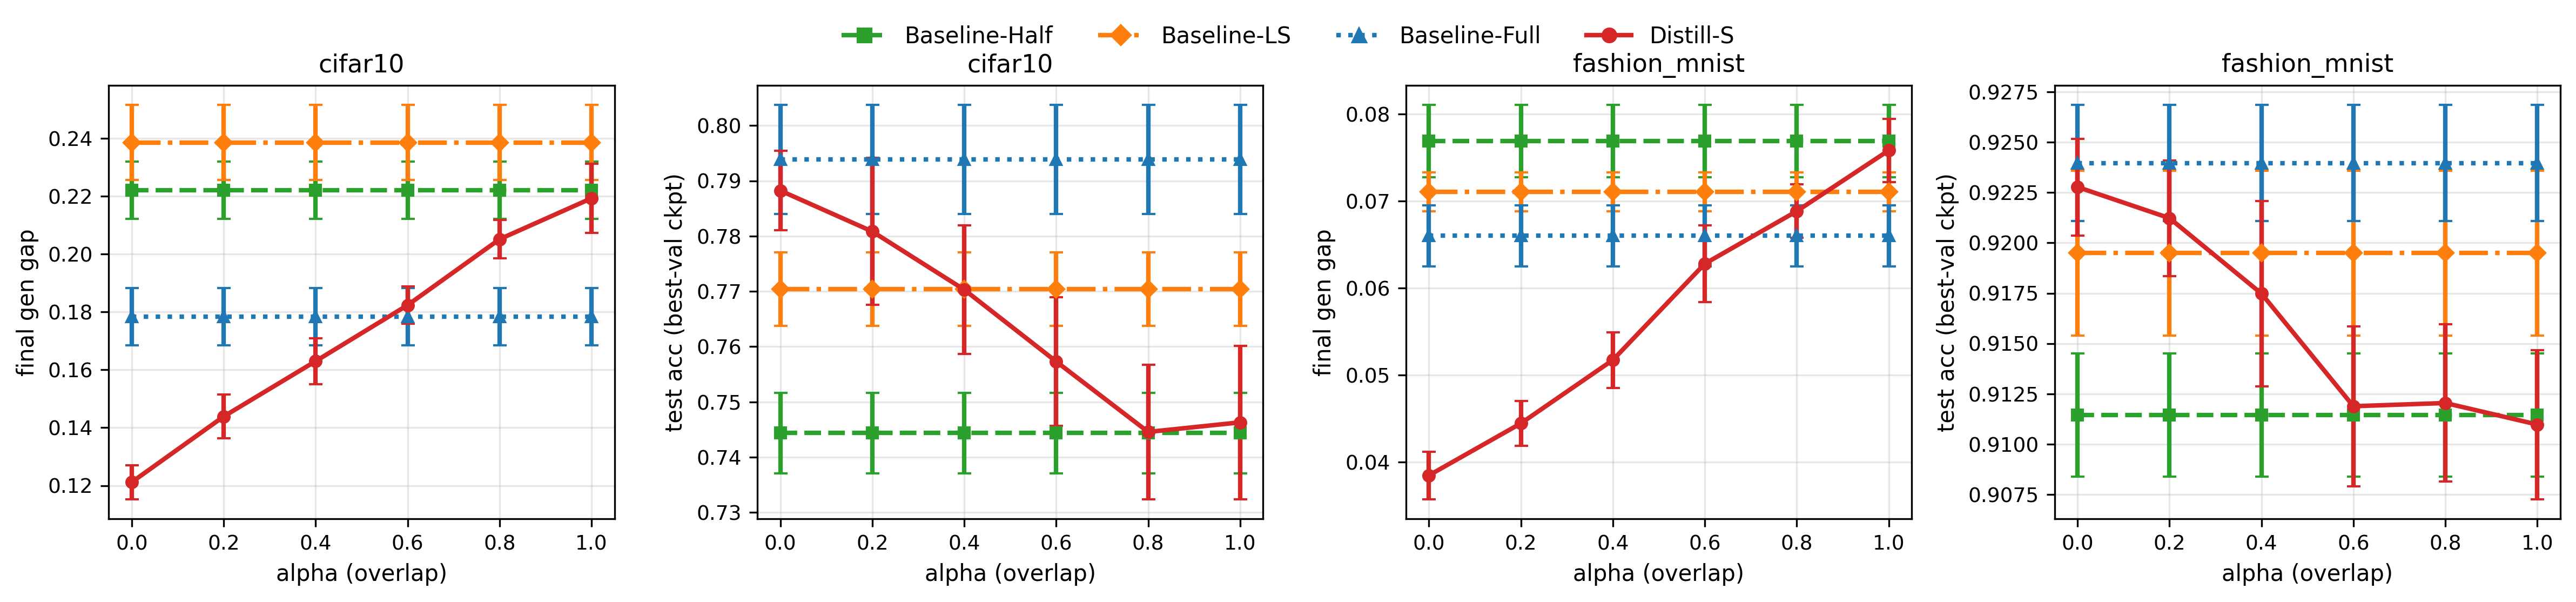
\includegraphics[width=0.98\textwidth]{results_ext/figs/fig_image_summary.png}
  \caption{Image benchmarks (Fashion-MNIST, CIFAR-10): final
           generalization gap (left panel per dataset) and test accuracy
           (right panel) versus overlap ratio $\alpha$ ($n=20$ seeds,
           error bars $\pm 1$ std).}
  \label{fig:images}
\end{figure*}

\subsection{Robustness to Teacher--Student Data Allocation}

\begin{figure*}[t]
  \centering
  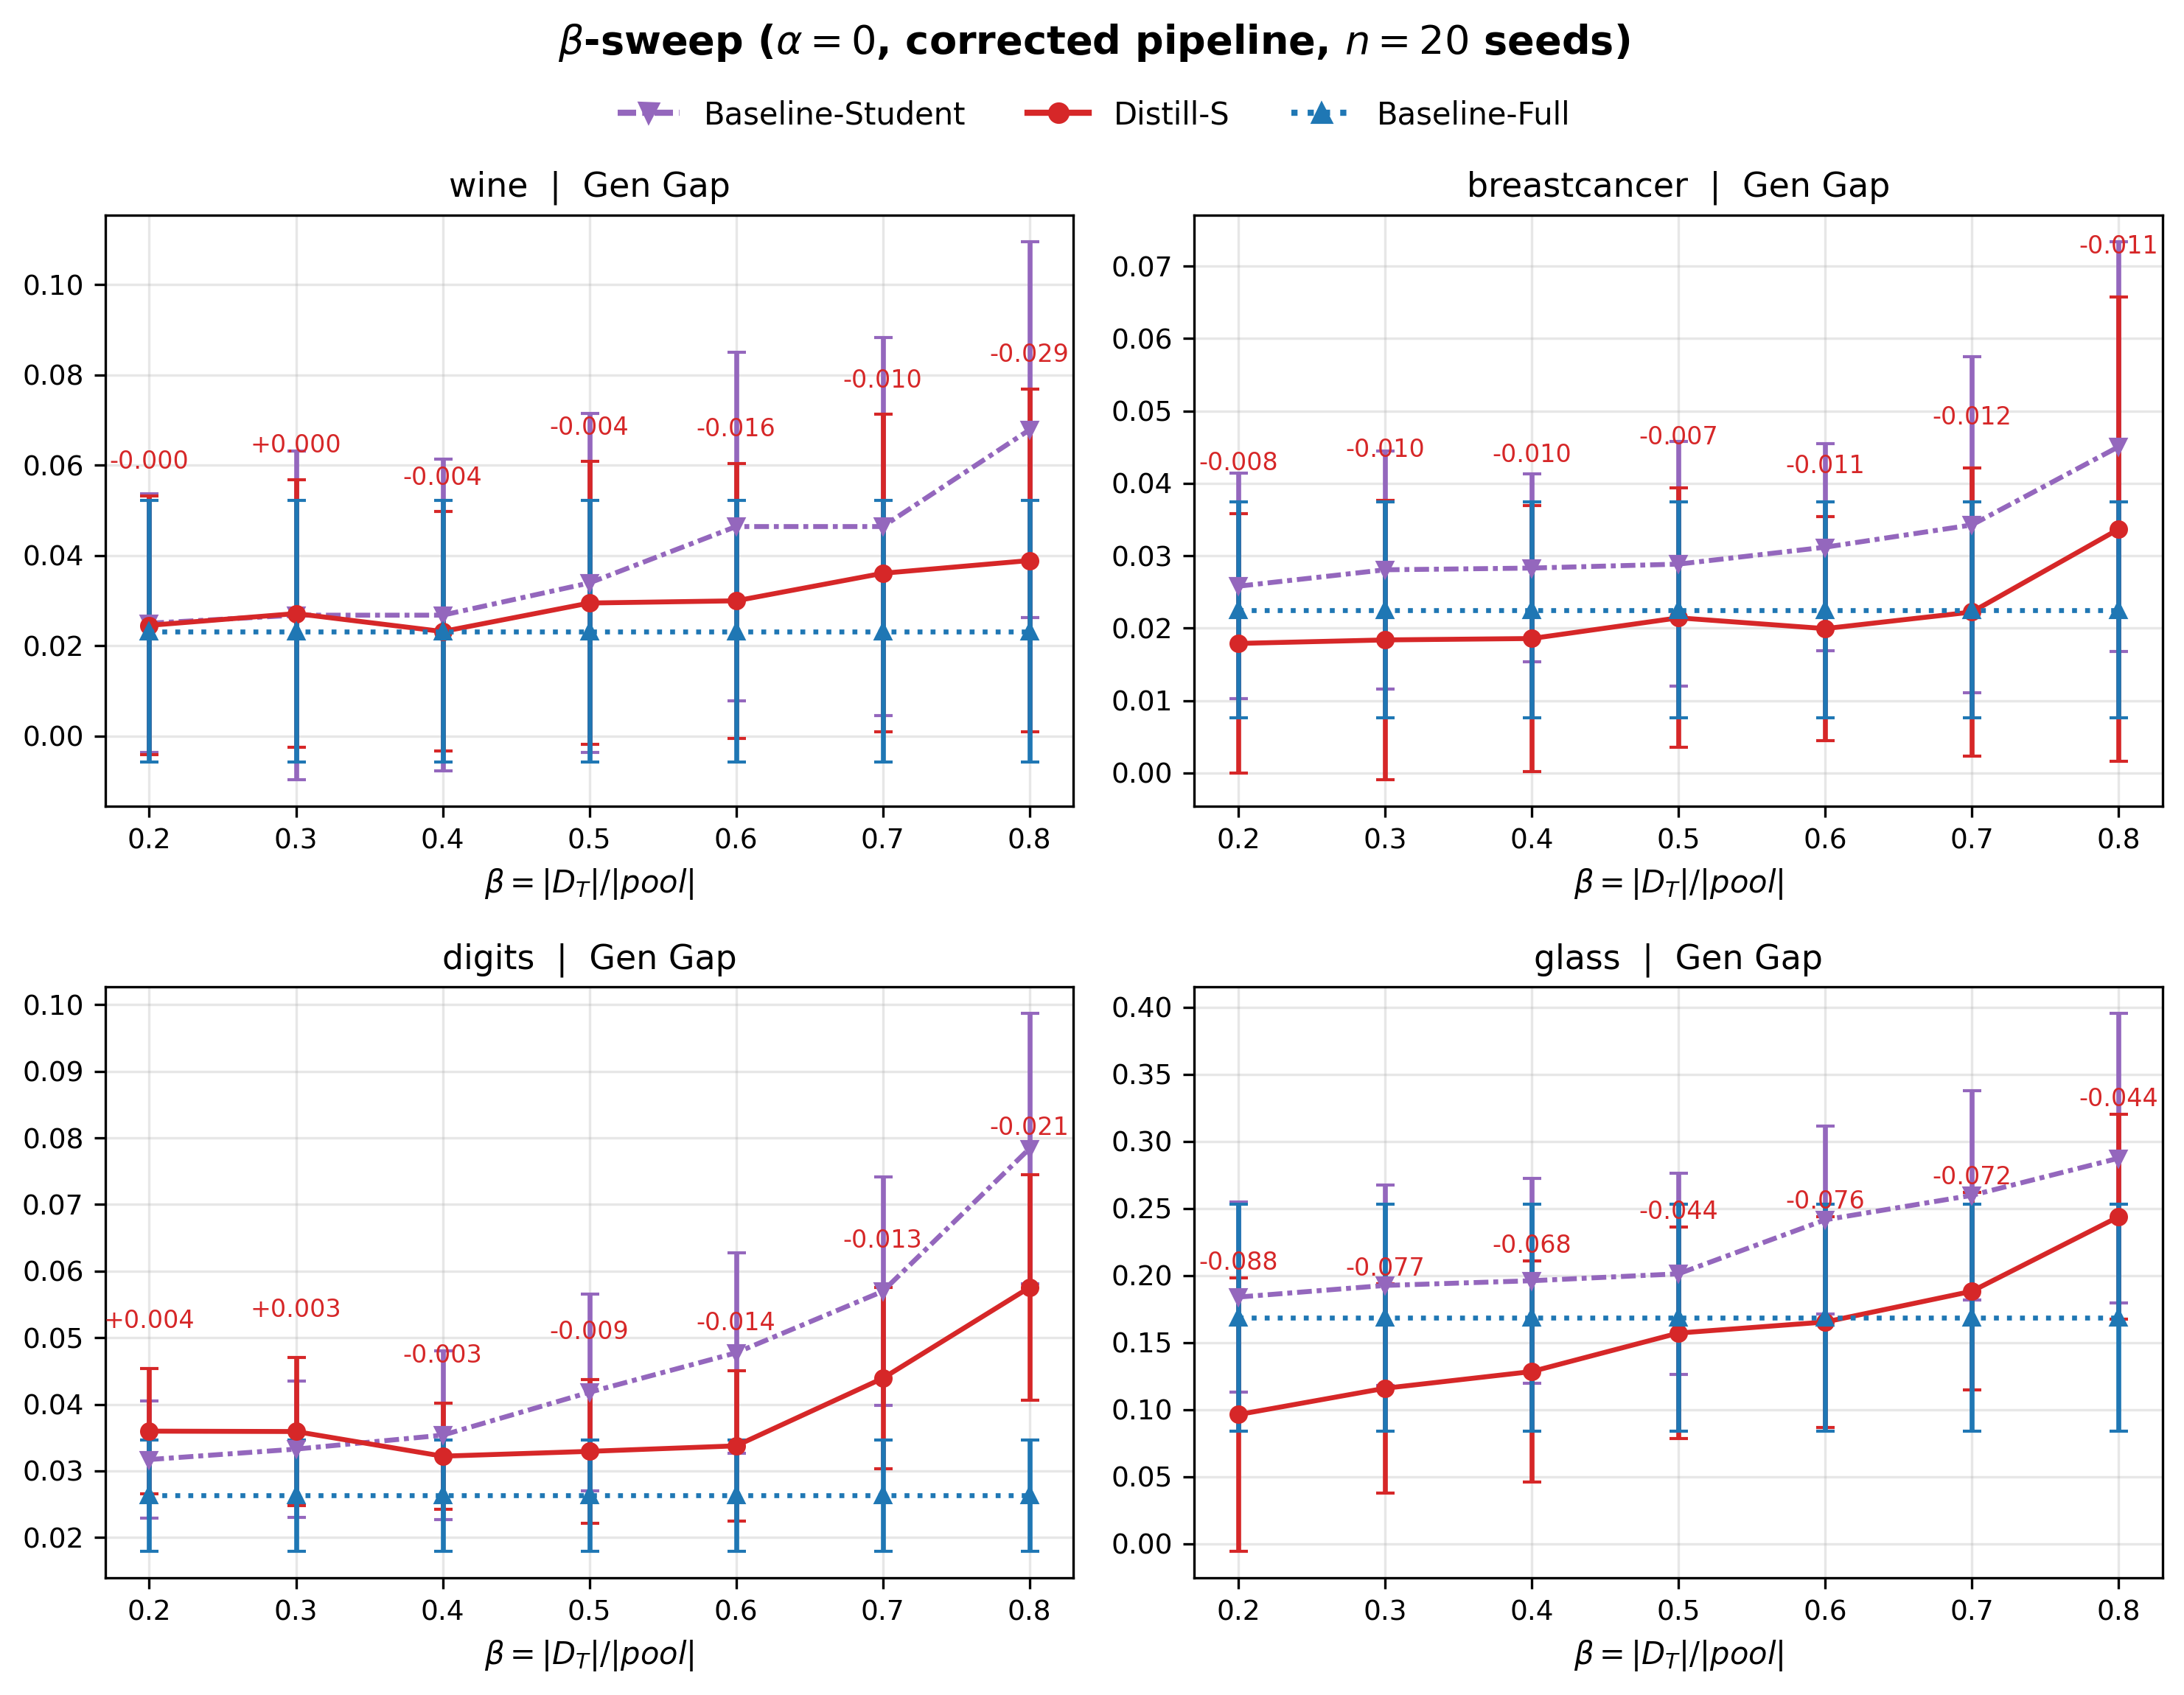
\includegraphics[width=0.85\textwidth]{results_ext/figs/fig_beta_sweep.png}
  \caption{Final generalization gap under different teacher--student
           allocation ratios $\beta$ ($\alpha{=}0$), all four tabular
           datasets, corrected pipeline, $n=20$ seeds, error bars
           $\pm1$~std. Distill-S is compared with the student-size-matched
           hard-label baseline (Baseline-Student); red annotations show the
           Distill-S $-$ Baseline-Student difference.}
  \label{fig:beta_sweep}
\end{figure*}

Figure~\ref{fig:beta_sweep} extends the allocation study to all four tabular datasets. On Glass the gap reduction is significant at every allocation except $\beta{=}0.5$ and $\beta{=}0.8$ (Holm-adjusted $p\le0.016$; $\Delta$ from $-0.088$ at $\beta{=}0.2$ to $-0.072$ at $\beta{=}0.7$), and on Breast Cancer the benefit is small but consistently negative ($\Delta\in[-0.012,-0.008]$, significant for $\beta\ge0.6$). Digits exhibits a minimum-teacher-pool effect: at $\beta{=}0.2$ the distilled student is slightly worse ($-0.012$ test accuracy, Holm $p{=}0.006$), whereas from $\beta{=}0.5$ the benefit turns positive and grows ($\Delta_{\mathrm{gap}}{=}-0.021$, $r{=}-1.0$, Holm $p<10^{-4}$ at $\beta{=}0.8$); Wine remains statistically flat throughout. At $\beta > 0.6$, both Distill-S and Baseline-Student exhibit increasing generalization gaps due to student data scarcity, suggesting that a minimum student sample size is a prerequisite for effective distillation---a constraint consistent with known sample-efficiency requirements in knowledge distillation more broadly.

Although the minimum gap occurs at a particular allocation ratio, this setting is not necessarily the most practically meaningful: in many applications, the size of the teacher's training set is constrained by data availability rather than freely chosen.


\subsection{Does Complementary KD Work?}
\label{sec:sep}


The experiments above suggest that complementary KD exerts a regularization effect. The key question is whether this effect comes from the teacher's complementary knowledge or merely from the smoothing induced by soft labels.
Table~\ref{tab:ls_comparison} compares Distill-S, Label Smoothing (LS), and
Baseline-Half at $\alpha{=}0$ (fully complementary partition) across four datasets.

\begin{table}[b]
\centering
\caption{Comparison with label smoothing at $\alpha{=}0$. Values are final
         generalization gaps; lower is better. Bold indicates the lowest gap
         for each dataset. $p$-values compare Distill-S with LS (paired
         Wilcoxon, Holm-adjusted within the metric family across datasets
         and $\alpha$; $^{*}p{<}0.05$).}
\label{tab:ls_comparison}
\setlength{\tabcolsep}{6pt}
\begin{tabular}{lcccc}
\toprule
Dataset & Baseline-Half & LS & Distill-S & $p$ \\
\midrule
Wine         & 0.0339 & 0.0304 & \textbf{0.0295} & 0.50\\
BreastCancer & 0.0288 & 0.0310 & \textbf{0.0214} & 0.16\\
Digits       & 0.0418 & \textbf{0.0256} & 0.0321 & 0.065\\
Glass        & 0.2012 & 0.2126 & \textbf{0.1570} & 0.014$^{*}$ \\
\bottomrule
\end{tabular}
\end{table}

On Glass, Distill-S yields a substantially smaller generalization gap than
Baseline-LS ($0.157$ vs.\ $0.213$), and this advantage survives Holm
correction. On Breast Cancer and Wine the gap of Distill-S is also lower
than that of LS, though the difference is not significant after correction
within the conservative across-dataset family. On Digits, LS achieves the
lowest gap and the highest test accuracy, confirming that generic
soft-target smoothing can be the stronger regularizer when the teacher
adds little instance-specific information (Section~\ref{sec:teacher}).
Beyond the gap, the proper predictive metrics in
Table~\ref{tab:test_metrics} sharpen this comparison: on Wine, Breast
Cancer, and Digits, Distill-S dominates LS on NLL and ECE at
Holm-adjusted $p<0.001$, indicating that the advantage of complementary
KD over generic smoothing is clearest in the quality of the predicted
distribution rather than in accuracy alone.


However, on Digits, Baseline-LS performs better than Distill-S. To probe a possible explanation, we measure the linear and local separability of each dataset.

\begin{table*}[t]
\centering
\caption{Dataset-level separability proxies. LDA 5-CV and 1-NN 5-CV report
         mean accuracies under 5-fold cross-validation using a linear
         discriminant classifier and a 1-nearest-neighbor classifier,
         respectively. Lower LDA accuracy suggests less linear separability,
         while lower 1-NN accuracy suggests stronger local class overlap.}
\label{tab:separability}
\setlength{\tabcolsep}{7pt}
\begin{tabular}{lcccc}
\toprule
Dataset & Classes & LDA 5-CV & 1-NN 5-CV & Distill-S vs.\ LS \\
\midrule
Wine         & 3 & 0.972 & 0.950 & $\approx$ (n.s.) \\
BreastCancer & 2 & 0.960 & 0.951 & Distill-S $>$ LS (NLL/ECE) \\
Digits       & 10 & 0.907 & 0.943 & LS $>$ Distill-S (acc., gap) \\
Glass        & 6 & 0.603 & 0.697 & Distill-S $>$ LS (gap) \\
\bottomrule
\end{tabular}
\end{table*}

Table~\ref{tab:separability} reports the mean accuracy of the two separability proxies on each dataset.
Glass is the only dataset where both proxies indicate poor separability,
consistent with its being the strongest beneficiary of complementary
distillation.

The strong separability of Wine and Digits corresponds to a regularization effect of Distill-S that is similar to or weaker than that of Baseline-LS. However, Breast Cancer is also highly separable, yet complementary KD remains effective. Thus, the current experiments do not provide a complete theoretical explanation. A plausible interpretation is that low separability may make complementary KD more likely to be beneficial, but high separability does not guarantee ineffectiveness; in highly separable regimes, the outcome may also depend on teacher soft-label quality, the number of classes, and calibration.

\paragraph{Difficulty, not modality.}
The separability reading makes a testable prediction: a genuinely hard
tabular dataset should behave like the image benchmarks rather than like
the easy tabular ones. We therefore repeat the $\alpha$-sweep on Yeast
(1{,}484 samples, 8 features, 10 classes, highly
imbalanced)~\citep{yeast}, whose MLP ceiling ($\approx 0.59$ test
accuracy) is close to that of Glass. The image pattern reappears: at
$\alpha{=}0$, complementary KD reduces the gap from $0.090$ to $0.063$
($\Delta{=}-0.027$, 95\% CI $[-0.037,-0.017]$, Holm-adjusted $p{=}0.002$,
$r{=}-0.90$), improves test accuracy by $1.0$ points ($p{=}0.028$,
$r{=}0.76$) and NLL ($p{<}10^{-3}$), and beats label smoothing on the
gap in all 20 seeds ($r{=}-1.0$, $p{<}10^{-4}$)---while LS itself
\emph{increases} the gap relative to the hard-label baseline ($0.111$
vs.\ $0.090$). The student ($0.593$) again exceeds its teacher
($0.569$), and the disagreement rate ($19.6\%$) falls between CIFAR-10
($13.3\%$) and Glass ($23.0\%$). Including Yeast, the seven
$\alpha{=}0$ dataset-level points remain monotonically related in the
disagreement--benefit sense (Spearman $\rho{=}0.786$, $p{=}0.036$,
$n{=}7$). The benefit is thus governed by task difficulty rather than by
data modality: hard datasets---tabular or image---show accuracy and NLL
gains alongside the gap reduction, whereas easy tabular datasets show a
near-pure regularization effect.



\section{Discussion}

An important observation is that, on the original tabular benchmarks, Distill-S shows no consistent improvement in validation or test accuracy relative to Baseline-Half/Baseline-Student, although the image benchmarks (Section~\ref{sec:images}) and the Yeast probe (Section~\ref{sec:sep}) show clear test-accuracy gains. This is consistent with the role of soft labels as a regularizer: they reshape the training objective but do not increase the number of training samples available to the student. Importantly, the test-set analysis (Section~\ref{sec:test}) shows that the distilled student improves the negative log-likelihood on all four datasets while preserving calibration, so the regularization is not a mere suppression of training accuracy.

\paragraph{The regularization effect of KD}

In the $\alpha$-sweep experiment discussed in Section~\ref{Effect}, Distill-S generally exhibits a smaller generalization gap than Baseline-Half. The stronger the complementarity between teacher and student data, the larger the reduction in this gap, and this trend appears from the early stages of training. This suggests that teacher soft labels can act as a regularizer when they encode inter-class structure not directly observed by the student, even though---on these tabular datasets---the gain in prediction accuracy remains close to zero.

The label-smoothing comparison further clarifies the nature of this
regularization effect. On the proper predictive metrics, the contrast is
decisive: Distill-S dominates Baseline-LS on NLL and ECE on three of four
datasets at Holm-adjusted $p<0.001$, and on Glass it retains the only
gap-level advantage that survives correction. However, the Digits result
shows that the advantage is not universal: when teacher-provided soft
labels carry little information beyond the student's own data
(Section~\ref{sec:teacher}), generic confidence smoothing can be the
stronger regularizer. Thus, complementary KD should be viewed as a
conditional regularization mechanism rather than a strict replacement for
label smoothing.

\paragraph{Robustness}

The regularization effect persists across teacher--student allocation
ratios $\beta$ whenever the student retains sufficient data, across
label-smoothing strengths $\varepsilon$, across distillation temperatures
and mixing weights at their predictive optimum, and across teacher
capacities (Sections~\ref{sec:sensitivity} and~\ref{sec:teacher}); image
benchmarks (Section~\ref{sec:images}) extend the protocol beyond small
tabular data. The sensitivity analysis also yields a methodological
caution: configurations that inflate the soft-label weight reduce the
training--validation gap while degrading test accuracy and NLL, so
gap-based evidence alone can overstate the benefit of distillation.


\paragraph{Limitation and Future Work}

The zero effect on Wine indicates that the complexity of the task itself is a prerequisite: for linearly separable problems, the inter-class structure can already be recovered from any subset, and complementary soft labels provide no additional gain.

The separability analysis in Section~\ref{sec:sep} should be interpreted as
exploratory rather than definitive. Poor separability appears consistent
with stronger gains from complementary KD on Glass, but it does not fully
explain all cases: Breast Cancer remains highly separable while still
favoring Distill-S, whereas Digits favors label smoothing. The
teacher--student agreement analysis (Section~\ref{sec:teacher}) offers a
more direct proxy---the fraction of soft labels encoding structure the
student has not recovered---and future work should examine teacher
calibration, predictive entropy, and class-count effects as additional
moderators of the Distill-S--LS tradeoff, together with stratified
overlap construction and the asymmetric regime $\beta \neq 0.5$ with
$\alpha > 0$. More broadly, the teacher--student disagreement rate
could be operationalized as a model-relative difficulty measure of a
dataset---harder datasets inducing larger complementary-data
advantages---which would turn the diagnostic quantity identified here
into an a priori selection rule between complementary KD and label
smoothing.

The same quantity also suggests an iterative extension: treat each distilled student as the next generation's teacher, re-draw a complementary ($\alpha{=}0$) partition every generation, and iterate while the disagreement on non-overlapping samples remains above a threshold. Holding the pool fixed bounds the expected gain by full-data training, so the decaying disagreement rate doubles as a model-relative stopping criterion---in contrast to pool-growing self-training such as the noisy student~\citep{xie2020noisy}, where injected pseudo-labelled data raises the ceiling each round. Scaling this partition-based generational loop to larger models and pools would connect the overlap framework to recent work on iterative self-improvement loops.

The observed relationship between data complementarity and distillation-induced generalization gap suggests a potentially useful diagnostic application: given a deployed student model and access to its teacher, the magnitude of the residual generalization gap --- measured under controlled partition structures --- may serve as a proxy for estimating the degree of overlap between teacher and student training distributions. This could inform data auditing or privacy-preserving federated learning scenarios where direct inspection of either party's dataset is unavailable. We leave the formalization of this inference framework as future work.


\section*{Data Availability}

The experimental code and related materials are available at
\url{https://github.com/leyi2014858504-glitch/Complementary-KD/tree/main}.

\section*{Declaration of Generative AI and AI-assisted Technologies In the Writing Process}


During the preparation of this work, the author used Perplexity Deep Research, DeepSeek, and other similar large
language models to improve the language and readability of the manuscript. For the experiments, the author
used large language models to assist in writing experimental scripts and generating statistical and plotting scripts based
on result naming conventions. However, the author did not use an LLM to directly
generate figures; all statistical results were computed solely with Python scripts and reviewed by the author.

\printcredits

%% Loading bibliography style file
%\bibliographystyle{model1-num-names}
\bibliographystyle{cas-model2-names}

% Loading bibliography database
\bibliography{cas-refs}

% Biography
%\bio{}
% Here goes the biography details.
%\endbio

%\bio{pic1}
% Here goes the biography details.
%\endbio

\end{document}
